\documentclass[a4paper,10pt]{article}
\usepackage[utf8]{inputenc}
\usepackage[english,russian]{babel}
\usepackage[top=2cm,bottom=3cm,left=0.5cm,right=2cm,nohead]{geometry}
\usepackage{multicol}
\usepackage{graphicx}

\graphicspath{{images/}}

\begin{document}
\section*{задачи по структуре программы}
\begin{enumerate}
    \item Чем отличается директива equ и '=' \par
    ничем
    \item в каком сегменте я могу написать equ \par
    в любом в том числе вне сегмента
    \item Чем отличается и какие ошибки произойдут и на каком этапе
    \begin{multicols}{2}
\begin{verbatim}
.code
    N equ 8
    mov N, eax
\end{verbatim}
        \columnbreak
\begin{verbatim}
.const
    N dd 8
.code
    mov N, eax
\end{verbatim} 
    \end{multicols} \par
N equ 8 - макрос что подставит 8 во время компиляции и не увидев инструкции imm|reg (таких не бывает) выдаст ошибку \\
в втором же случае ошибка произойдёт во время счёта(исполнения загружаемого файла), так как наших прав (пользователя) недостаточно чтобы получть доступ к записи сегмента .const \\

    \item Опишите секцию .data? \par
В секции описываются неициализированные данные ? - отмеченные в файле asm вопросительным знаком запись зараннее игнорируется при трансляции\\
    \item программа компилируется стандартно "ml /c /coff /Fl main.asm" будет ли ошибка?
\begin{verbatim}
.data?
    msg db 'Hello World', 0
\end{verbatim}
Нет не будет, случится лишь предупреждение \\
    \item опишите .stack, может ли эта секция встретиться в неглавном модуле? \par
Секция stack определяется в главном модуле, она задаёт размер стека на начало счёта, впоследствии его можно динамически расширить сдвигая esp, если не будет .stack в главном модуле то при линковке всё равно отведётся страница (4КБ) .stack других модулей проигнорируется
    \item Бородоченкова 6.1 (на правильность написания адресных выражений) \par
    Неправильные: б, г, д, е, з, и, к, л, н, п, т, у \par
    \begin{figure}[htbp]
        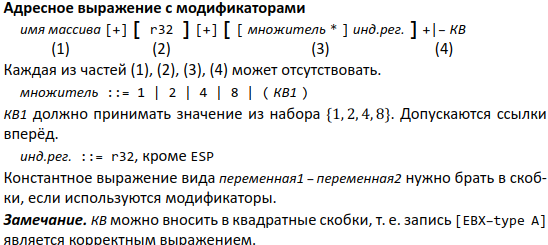
\includegraphics[width=0.5\textwidth]{скрин с бородаченковой.png}
        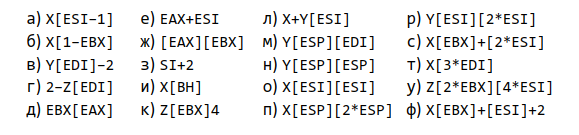
\includegraphics[width=0.5\textwidth]{скрин задачи.png}
    \end{figure}
    \item Бородоченкова 7.1 a) б) 7.2 а) 7.6 д) - макет для решения 7.2 7.6 в директории, задача усложенена: сколько людей имеют средний балл выше 4.6?
    \item На листочке опишите структуру вашего холодильника (творчески)
    \item Выпишите весь вывод
\begin{verbatim}
include console.inc

metadata STRUC
    timestamp dq ?
    author db '6MaXXaM6',0
    testdata db 0FFh
metadata ENDS

.data
    typ db 5 dup ('6MaXXaM6'),0
    x metadata <12>, <23>
.code
start: 
    outu length metadata.author
    outu length typ
    outu lengthof metadata.author
    outu sizeof metadata.author
    outu size metadata.author
    outu sizeof metadata
    outu sizeof x
    outstrln offset x.author
    outu x.timestamp
    lea eax, x
    outu [eax+metadata.timestamp]
    exit
end start
\end{verbatim}
1 5 9 9 1 18 36 6MaXXaM6 12 12
\end{enumerate}

\end{document}